\documentclass{article}
\usepackage[utf8]{inputenc}
\usepackage[left=1cm, right=1cm, top=2cm, bottom=2cm]{geometry}
\usepackage{graphicx}
\usepackage{caption}
\usepackage{subcaption}
\usepackage{amsmath}
\usepackage{booktabs} % Used for professional table formatting
\usepackage{float}
\usepackage[colorlinks=true, urlcolor=blue, linkcolor=blue, citecolor=blue]{hyperref}
\usepackage{cleveref}

\title{Store Sales Data and Modeling Report}
\author{Gabriel Loos}
\date{March 2026}

\begin{document}

\maketitle

\section{Introduction}

In this project, we will be working with the Store Sales Time Series data set from Kaggle. The data set can be found at \url{https://www.kaggle.com/competitions/store-sales-time-series-forecasting}. The goal of the competition is to accurately predict the sales for the last sixteen days of August 2017. The provided data for training contains all the sales prior to the test dates, dating back to the beginning of 2013. The competition uses root mean squared logarithmic error (RMSLE) as its evaluation metric.

\section{EDA}

Since the data has already been provided on Kaggle, there is minimal cleaning that must be done. The relevant provided files are train.csv, test.csv, holidays\_events.csv, stores.csv, and oil.csv. Of all the files, only oil.csv contains missing values. About $30.88\%$ of the oil values are missing for all the given dates. It is also seen in \Cref{fig: oil} that the oil prices start off around $100$ but at the end of $2014$ drop to be around $50$. From \Cref{fig: log1p(sales)}, one sees that the sales, on average, seem mostly unaffected by this drop. For these reasons, and in order to keep our models more simple, we choose not to utilize the oil data.

\begin{figure}[H]
    \centering
    \captionsetup{justification=centering}
    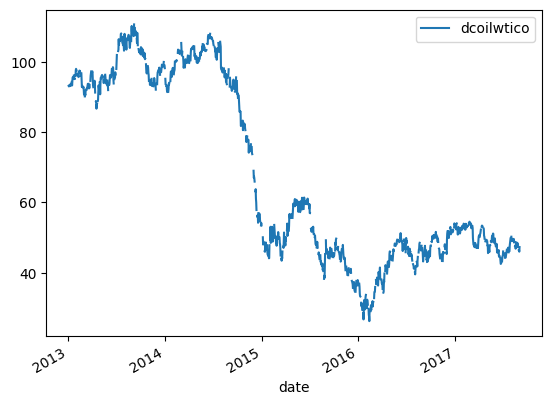
\includegraphics[width=0.5\textwidth]{images/oil.png} 
    \caption{Oil Prices}
    \label{fig: oil}
\end{figure}

\begin{figure}[H]
    \centering
    \captionsetup{justification=centering}
    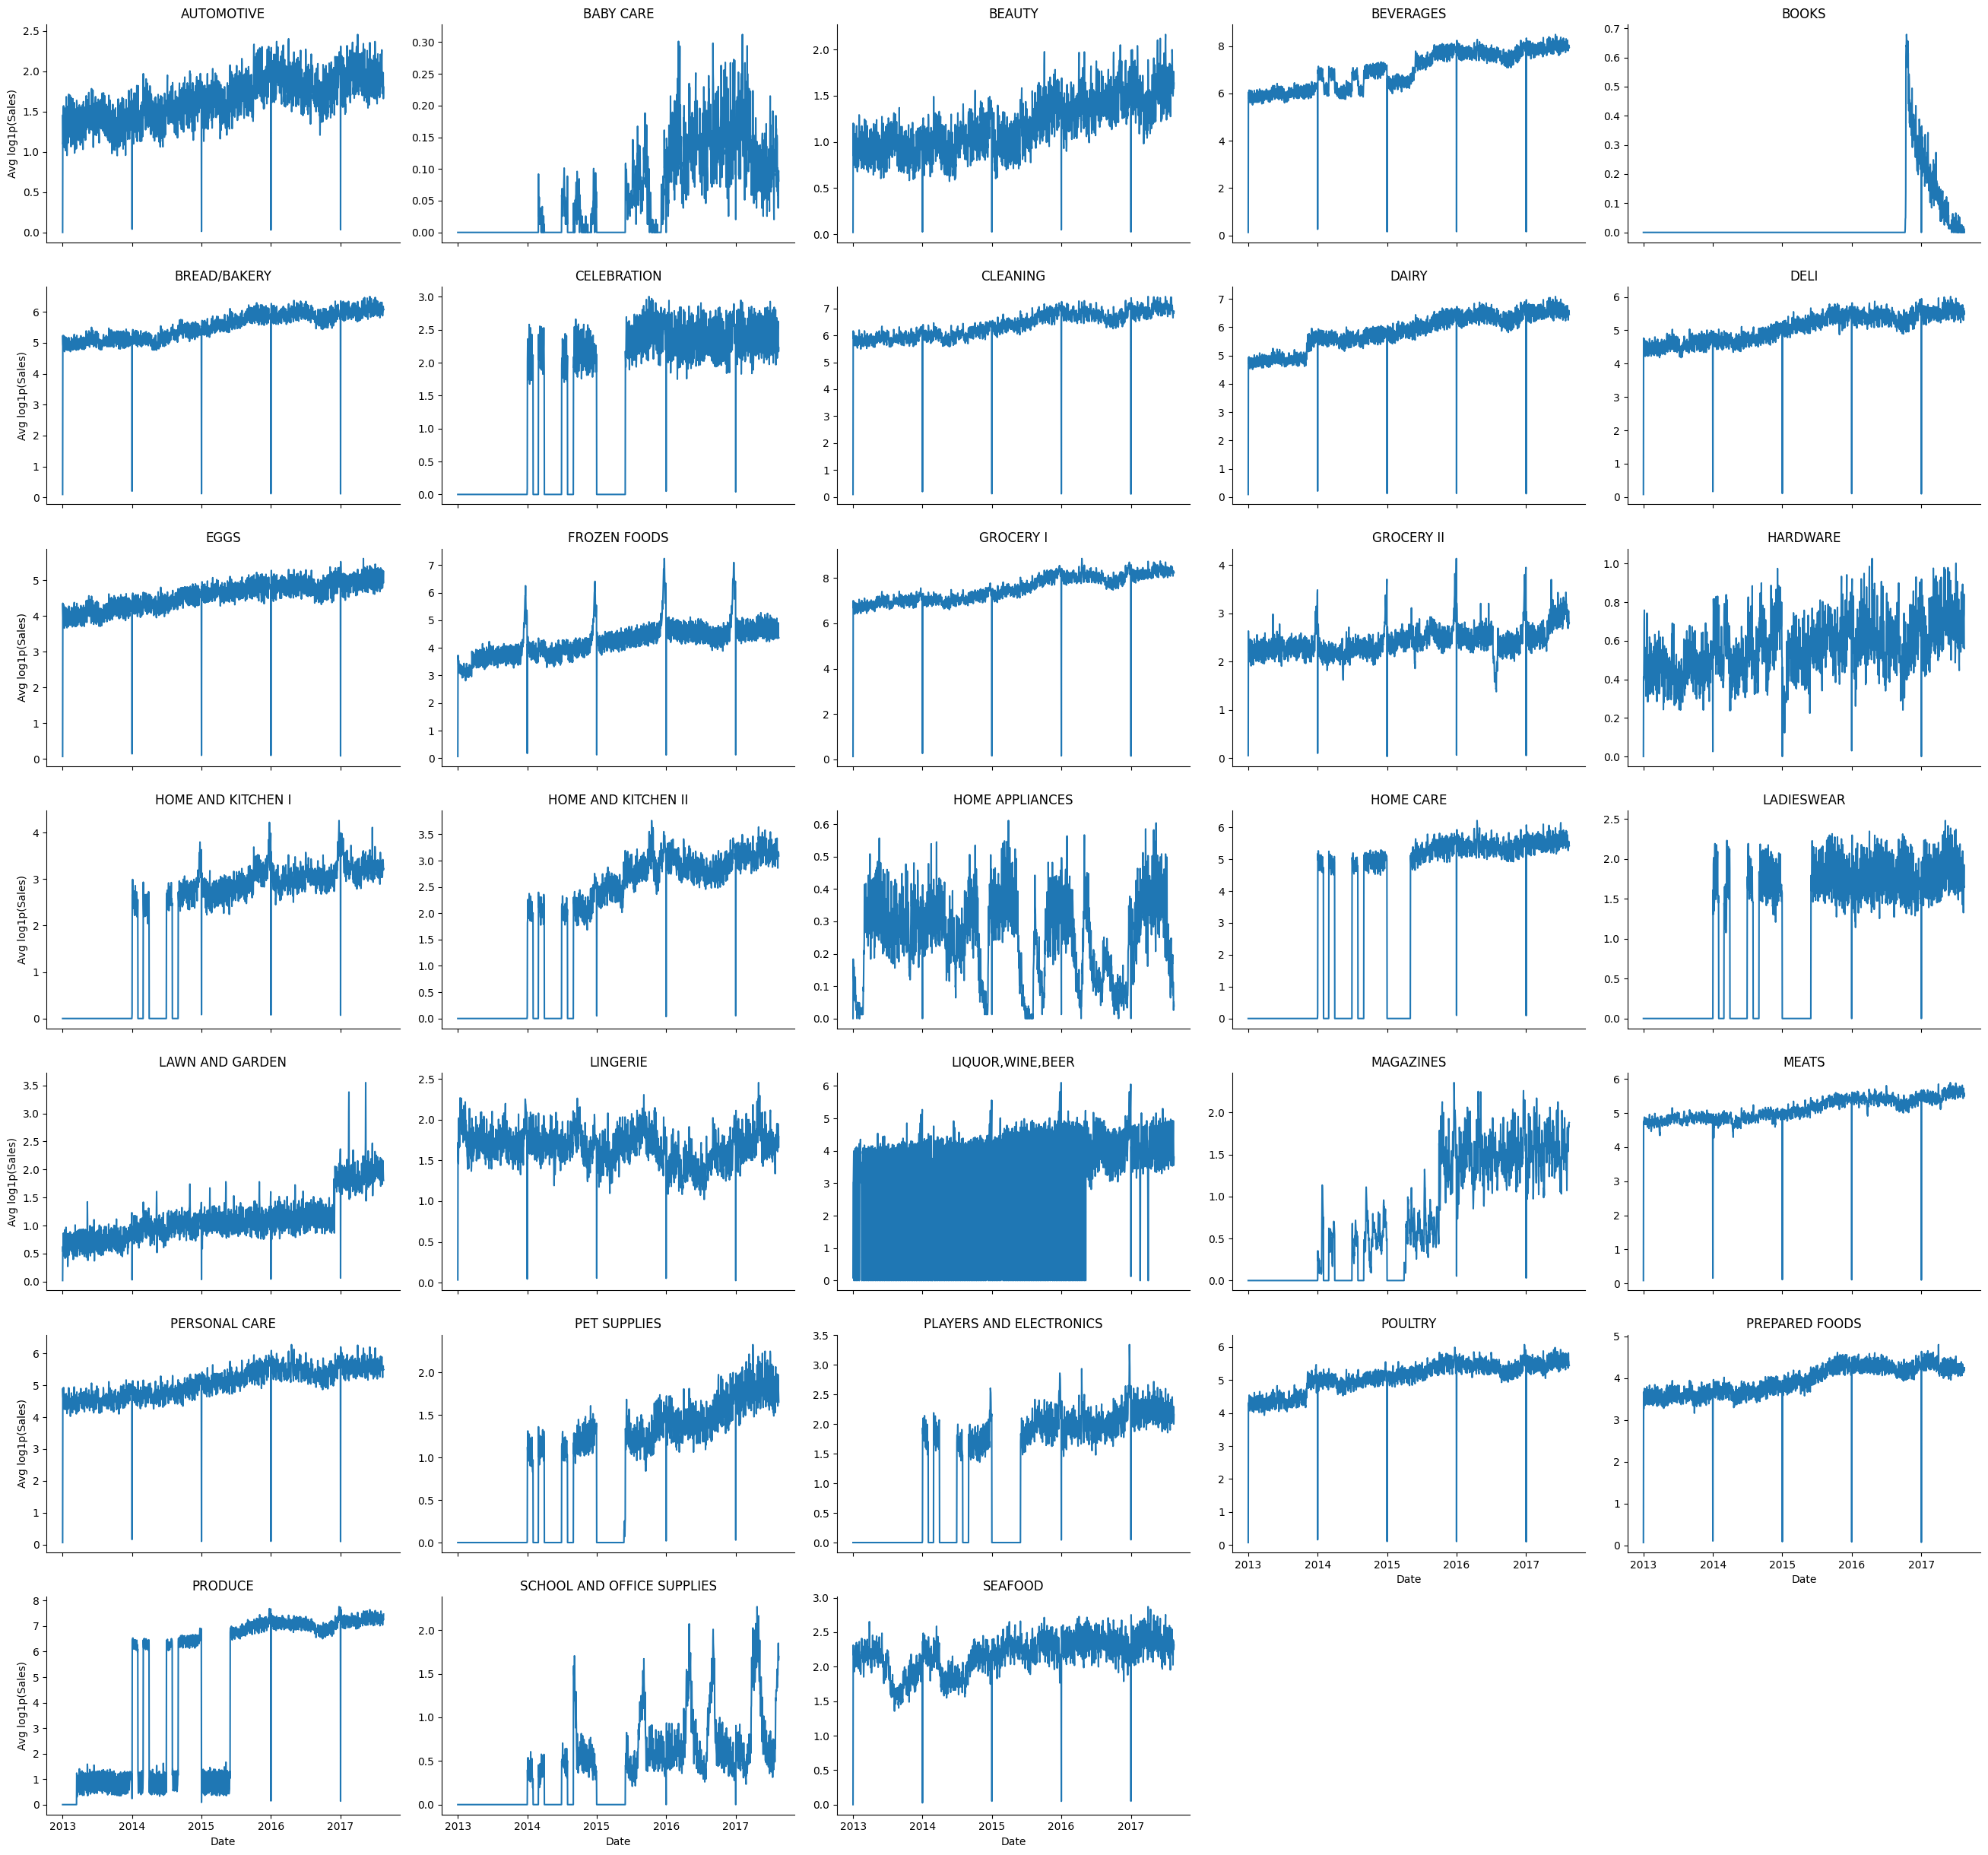
\includegraphics[width=\textwidth]{images/sales.png} 
    \caption{Average log1p(sales) by family and date}
    \label{fig: log1p(sales)}
\end{figure}

The last bit of analysis on the data that we do is examining the relationship between the store numbers, clusters, and types. Each store has a unique number that identifies it. There are $54$ different stores. Each store then falls into one of $17$ clusters and one of $5$ types. The only cluster which contains stores of different types is cluster $10$, which contains stores of type B, D, and E. Every other cluster only contains stores of the same type. Thus, we will view clusters as being more specific than types.

\section{Feature Engineering}

For all models, we log-transformed the target variable using \texttt{log1p(sales)}. This approach provides two main advantages: (1) it reduces the skewness of the sales data, and (2) computing the RMSE on \texttt{log1p(sales)} perfectly aligns with the competition's evaluation metric of RMSLE. To obtain the final sales predictions, we simply applied the inverse transformation (\texttt{expm1}). Additionally, all models utilized the product family and store number as categorical features.

Starting with Model 2, we introduced the day of the week as a categorical variable, alongside sine and cosine transformations of the day of the year (with periods of $1$, $1/2$, and $1/3$ of a year) to capture seasonality. To account for external events, we included a boolean feature indicating if a date falls within a month of the April 16, 2016 earthquake. Because public sector wages are paid on the 15th and the last day of the month, we added a feature tracking the number of days since the last payday, as well as a calendar-based holiday indicator. Finally, we incorporated $16$-, $21$-, and $28$-day lags of the target variable. Since the Kaggle test set is $16$ days long, restricting our lags to $16$+ days allows us to forecast the entire window directly without relying on recursive predictions. The $16$-day lag represents the most recent available data, while the $21$- and $28$-day lags correspond to exactly three and four weeks prior, capturing weekly shopping habits.

For Model 4 and subsequent iterations, we included an interaction term between the product family and the number of items on promotion. This captures the reality that promotional sensitivity varies significantly by product category (e.g., a promotion on beverages might yield a different sales spike than one on books). 

Prior to building Model 5, we utilized Lasso regression to perform feature selection on various lag intervals, which led us to include additional $17$-, $18$-, $19$-, and $20$-day lags, alongside interaction and polynomial terms for most numeric features. These specific additions were exclusive to Model 5. 

For Models 6, 7, and 8, we experimented with different interaction terms to capture spatial and categorical nuances. Model 6 introduced an interaction between family type and store type; Model 7 used family type and store cluster; and Model 8 used family type and store number. These features were designed to account for the fact that specific product families sell differently depending on a store's specific region, size, or customer demographic.

\section{Modeling}

To establish a baseline (Model 1), we predicted the historical average of \texttt{log1p(sales)} for each unique combination of store and product family. Model 2 expanded on this by fitting independent linear regressions for each store-family pair, while Model 3 applied Ridge regression to these same groups to introduce regularization. However, while Models 2 and 3 achieved low RMSLE scores on our internal validation sets, they performed poorly on the hidden test set. This discrepancy strongly suggested overfitting and an inability to capture macro-level trends. Consequently, starting with Model 4, we transitioned to a global approach: training a single Ridge regression model across the entire dataset. For all models, prior to final evaluation, we clipped our predictions to bound them at zero, eliminating any impossible negative sales forecasts.

To determine the optimal regularization parameter ($\alpha$) for our Ridge regressions, we employed two distinct validation methodologies:
\begin{enumerate}
    \item \textbf{Out-of-Sample (OOS) Validation:} We isolated the final $15$ days of the training set to serve as a static validation holdout. The models were trained on all preceding data, and Bayes Search was utilized to select the $\alpha$ parameter that explicitly minimized the error (RMSLE) on this specific $15$-day testing window.
    \item \textbf{Time Series Cross-Validation (CV):} To prevent data leakage and evaluate performance across multiple time horizons, we used an expanding-window Time Series Split approach. We combined this with Bayes Search (and Grid Search for Model 3) to optimize $\alpha$ based on average performance across the folds. Crucially, the final $15$ days of the training data were completely excluded from these CV folds.
\end{enumerate}

After identifying the optimal $\alpha$ using both methods, we evaluated the models on the $15$-day holdout set (Validation RMSLE). Finally, we retrained the models on the entirety of the training data and generated predictions for the Kaggle test set (Test RMSLE). The results are summarized in \Cref{tab: Model Evaluation}. Note that Model 1 (the baseline) has no tunable $\alpha$ or validation scores, so only its final test score is reported. Similarly, Model 3 lacks a single global $\alpha$ since it consists of many independent local models.

\begin{table}[H]
\centering
\caption{Model Evaluation}
\label{tab: Model Evaluation}
\begin{tabular}{lcccccccc} 
\toprule
 & Model 1 & Model 2 & Model 3 & Model 4 & Model 5 & Model 6 & Model 7 & Model 8 \\ 
\midrule
OOS $\alpha$ & - & - & - & 0.0023 & 559948.6743 & 0.0067 & 0.0010 & 223.2250 \\ 
Validation RMSLE & - & 0.4906 & 0.4600 & 0.5200 & 0.5389 & 0.5090 & 0.5094 & 0.5091 \\ 
Test RMSLE & 1.31791 & 0.72757 & 0.67004 & 0.46885 & 0.48015 & 0.46614 & 0.46792 & 0.47324 \\ 
\midrule
CV $\alpha$ & - & - & - & 1952.1126 & 313963.0962 & 2111.7017 & 3332.6314 & 2728.3037 \\ 
Validation RMSLE & - & - & 0.4914 & 0.5369 & 0.5407 & 0.5352 & 0.5331 & 0.5301 \\ 
Test RMSLE & - & - & 0.62904 & 0.47383 & 0.47735 & 0.46953 & 0.46998 & 0.46822 \\ 
\bottomrule
\end{tabular}
\end{table}

As expected, the OOS Validation RMSLE is consistently lower than the CV Validation RMSLE, because the OOS $\alpha$ is explicitly tuned to minimize error on that exact $15$-day validation window. In contrast, the CV approach never exposes the model to the validation set during hyperparameter tuning. Interestingly, with the exception of Model 5, the optimal OOS $\alpha$ is significantly smaller than the CV $\alpha$, yet the final Test RMSLE scores remain comparable. 

Ultimately, while Model 6 with the OOS $\alpha$ achieved the best Test RMSLE score (the primary metric of the competition), it is likely overfit to the specific temporal dynamics of the final $15$ days of August. Based on the data in \Cref{tab: Model Evaluation}, Model 8 using the CV-derived $\alpha$ proved to be the most robust choice: it achieved a highly competitive Test RMSLE without explicitly overfitting to a single, static validation window.

\section{Summary}

To build the most robust and generalizable model for predicting store sales, we recommend utilizing a global Ridge regression approach (Model 8) with a cross-validated regularization parameter of $\alpha = 2728.3037$. This optimal model predicts \texttt{log1p(sales)} utilizing the following feature set:

\begin{enumerate}
    \item Product family (categorical).
    \item Store number (categorical).
    \item Day of the week (categorical).
    \item Sine and cosine transformations of the day of the year, utilizing periods of $1$, $1/2$, and $1/3$ of a year to capture seasonality (numeric).
    \item A boolean indicator for dates falling within one month of the April 16, 2016 earthquake (categorical).
    \item The number of days since the last public sector payday (numeric).
    \item Calendar holiday indicators (categorical).
    \item $16$-, $21$-, and $28$-day lags of \texttt{log1p(sales)} (numeric).
    \item An interaction term between the product family and the number of items on promotion (categorical).
    \item An interaction term between the product family and the store number (categorical).
\end{enumerate}

During the inference phase, the model outputs predictions in the transformed logarithmic space. To finalize the forecasts, one must first clip the outputs to bound all predictions at zero (eliminating negative predictions), and subsequently apply the inverse log transformation (\texttt{expm1}) to project the values back to their original sales scale.

\end{document}